\RequirePackage{plautopatch}
\RequirePackage[l2tabu, orthodox]{nag}

\documentclass[fontsize=12pt,platex,dvipdfmx,standalone]{jlreq}			% for platex
% \documentclass[uplatex,dvipdfmx]{jlreq}		% for uplatex

\usepackage[top=8truemm, bottom=8truemm, left=15truemm, right=15truemm]{geometry}

\renewcommand{\baselinestretch}{1.1}

\usepackage{graphicx}
\usepackage{bxtexlogo}
\usepackage{amsmath}
\usepackage{amssymb}
\usepackage{amsthm}
\usepackage{mathtools}
\usepackage{here}
\usepackage{pgfplots}
\usepackage{adjustbox}
\usepackage{ascmac}
\usepackage{fancybox}

\pgfplotsset{compat=1.18}

\usepackage{tikz}

\everymath{\displaystyle}

\let\Re\relax
\DeclareMathOperator{\Re}{Re}
\let\Im\relax
\DeclareMathOperator{\Im}{Im}

\theoremstyle{definition}
\newtheorem{thm}{定理}[section]
\newtheorem{dfn}[thm]{定義}
\newtheorem{prop}[thm]{命題}
\newtheorem{qst}[thm]{問}
\newtheorem*{qst*}{問題}
\newtheorem{rem}{注意}
\newtheorem*{rem*}{注意}
\newtheorem*{exq*}{例題}
\newtheorem*{ex*}{例}
\newtheorem*{ans*}{解答}

\renewcommand{\labelenumi}{(\arabic{enumi})}
\pagestyle{empty}

\begin{document}
\section*{中1数学 空間図形 第5回 ワークシート}
\vspace{-15.2mm}
\rightline{名前 \underline{\hspace{50mm}}}
\begin{itembox}[l]{本時の目標}
  円柱の見取図と展開図をかこう。
\end{itembox}

\vspace{-3mm}

\begin{enumerate}
\item  身の回りに円柱の形をしているものは,どのようなものがありますか?
\begin{screen}
  \vspace{6mm}
\end{screen}
  \item  長方形の$2$つの向かい合う辺を折らずに重ねるとどのような図形になるでしょうか?長方形の別紙の★の位置を重ねてみて確認しよう。
  
  \vspace{2mm}
  \begin{center}
\begin{adjustbox}{center}
  \begin{tikzpicture}
  % 長方形を描く
  \draw (0, 0) rectangle (4, 3);
  
  % ★マークを描く
  \node at (0.3, 1.5) {$\bigstar$};
  \node at (3.7, 1.5) {$\bigstar$};
\end{tikzpicture}
\end{adjustbox}
\end{center}

\item  円柱の展開図を作るためには,長方形にどのような図形をつけ加えればいいでしょうか?周りの人と相談しましょう。
\begin{screen}
  \vspace{7mm}
\end{screen}
\item  円柱の見取図と展開図を書きましょう。


\begin{center}
  \begin{adjustbox}{center}
    \begin{tikzpicture}
  % 1つ目の正方形を描く
  \draw (0, 0) rectangle (6, 6);
  \node at (3, -0.5) {見取図};
  
  % 2つ目の正方形を描く
  \draw (7, 0) rectangle (13, 6);
  \node at (10, -0.5) {展開図};
\end{tikzpicture}
  \end{adjustbox}
\end{center}
\item  円柱の展開図について,底面と側面はそれぞれどのような平面図形になりますか?下の表に書き入れて整理しましょう。
\begin{table}[H]
  \centering
  \begin{tabular}{c|c}
    円柱の面 & 平面図形 \\ \hline
    底面 & \hspace{40mm}\\
    側面 & \hspace{40mm}
  \end{tabular}
\end{table}
\item \hspace{5mm}
\vspace{-7.5mm}
\begin{minipage}[t]{0.5\textwidth}  % 左側の文章部分(幅の50%)
\vspace{-65mm}
 右のような,底面の直径が$3$cmで,高さが$5$cmの円柱があります。下の図でこの円柱の展開図を完成させましょう。\\
 (ただし、$1$マスの$1$辺の長さは$0.5$cmです。)
\end{minipage}%
\begin{minipage}[t]{0.5\textwidth}  % 右側のTikZ画像部分(幅の50%)
\begin{center}  %中央揃えにする
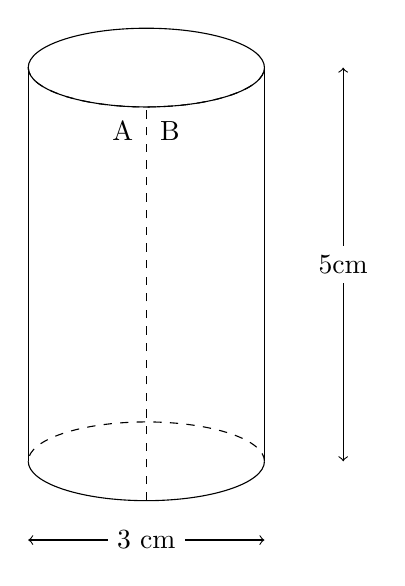
\begin{tikzpicture}

% 円柱の底面を描く
\draw (-1.5,0) arc (180:360:1.5cm and 0.5cm);
\draw[dashed] (1.5,0) arc (0:180:1.5cm and 0.5cm);

% 円柱の上面を描く
\draw (0,5) ellipse (1.5cm and 0.5cm);
\draw[dashed] (-1.5,5) arc (180:360:1.5cm and 0.5cm);

% 円柱の側面を描く
\draw (-1.5,0) -- (-1.5,5);
\draw (1.5,0) -- (1.5,5);

\draw[dashed] (0, -0.5) -- (0, 4.5);

\node at (-0.3, 4.2) {A};
\node at (0.3, 4.2) {B};

% 直径と高さのラベルを描く
\draw[<->] (-1.5, -1) -- (1.5, -1) node[midway, fill=white] {$3$ cm};
\draw[<->] (2.5, 0) -- (2.5, 5) node[midway, fill=white] {$5$cm};

\end{tikzpicture}
\end{center}
\end{minipage}

\begin{center}
  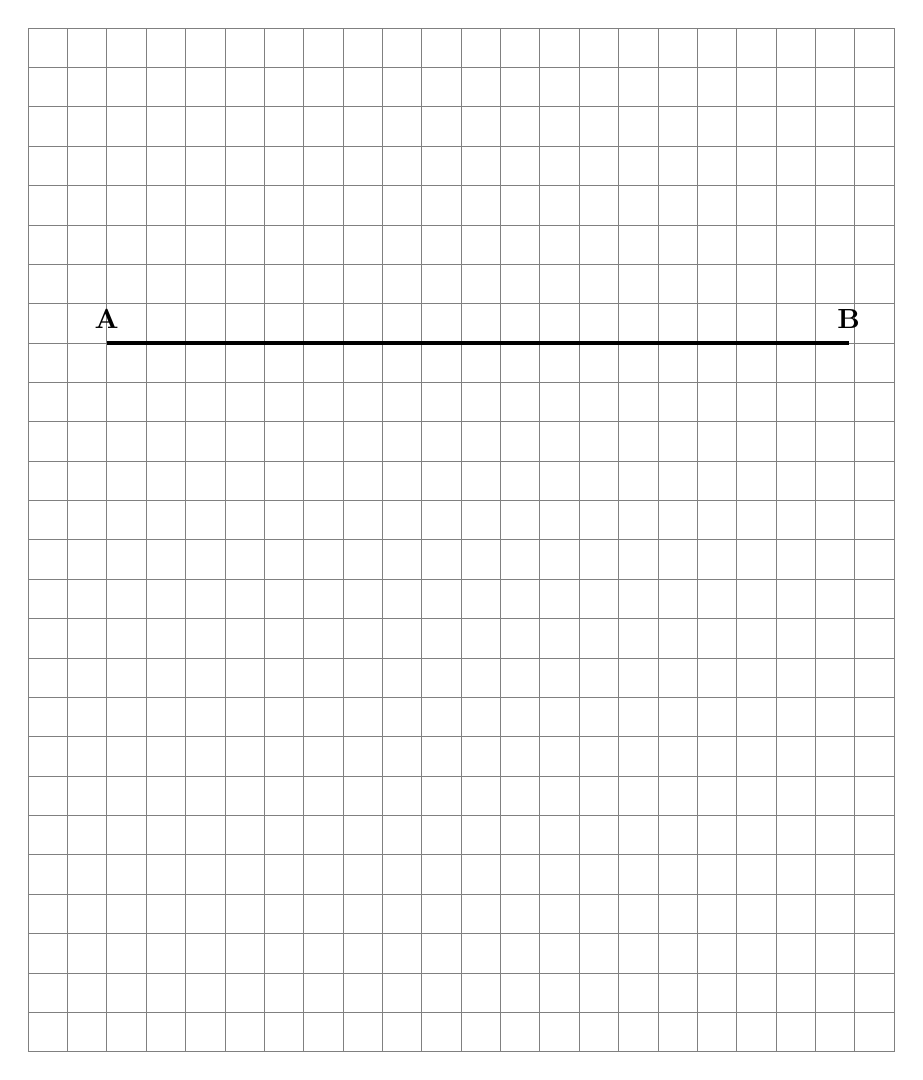
\begin{tikzpicture}
    \draw[step=0.5cm,gray,very thin] (0,0) grid (11,13);
    \draw[very thick] (1, 9) -- (10.42478, 9);
    \node at (1, 9.3) {\textbf{A}};
    \node at (10.42478, 9.3) {\textbf{B}};
    \end{tikzpicture}
\end{center}
\begin{itembox}[l]{メモ}
  \vspace{30mm}
\end{itembox}
\end{enumerate}

\begin{itembox}[l]{本時の感想}
  \vspace{10mm}
\end{itembox}

\end{document}
